\chapter{Low Complexity Multiply Accumulate Unit for Weight-Sharing Convolutional Neural Networks}

{\small \textbf{Authors}\\
James Garland and David Gregg\\ \\
IEEE COMPUTER ARCHITECTURE LETTERS\\VOL. 16, NO. 2, JULY-DECEMBER 2017}

\section{Proposed Method}

This is the first paper in which we are going to discuss about something that deals with both hardware and the pure model. Until now, we have been discussing only about technical improvements related to CNNs from a modeling perspective. For instance, we have talked a lot about number of layers, size of filters, pooling operations, how to better convolve etc. On the other hand here, we will debate on advantages of adopting a different tecnique to store weights, that is closer to the hardware. The idea is to propose a different way to perform the accumulation of the weights in the \textit{Multiply Accumulate Unit} (MAC). Recall that the multiply accumulate operation is the product between two numbers where the result is added to an accumulator, which is also known as Sum of Products (SOP). So instead of doing that, a different approach is proposed. Basically, for each weight that we have, we put its image (that is different from its original value) into a bucket with a fixed index. Until weights show up, we add their images to the right buckets. What we are doing is performing an accumulation. The next step now is to perform the multiplication between the image values stored into our buckets and the value of the weight of that bucket. By doing so we reduce a lot the number of operations that we should have done because we move from a multiplication accumulation problem to an addition based on array indexes. As this might be a little difficult to imagine, we provide an illustration of these accumulators in Figures \ref{fig:09_2} and \ref{fig:09_3}.\\

\begin{figure}[h!]
    \centering
    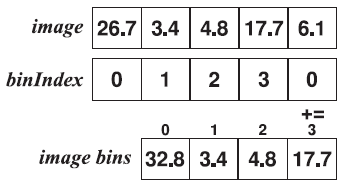
\includegraphics[scale=0.70]{images/09_2.png}
    \caption{Step 1: Accumulation of images.}
    \label{fig:09_2}
\end{figure}

\FloatBarrier

\begin{figure}[h!]
    \centering
    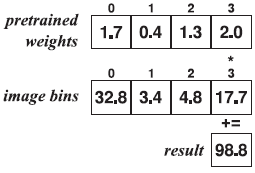
\includegraphics[scale=0.70]{images/09_3.png}
    \caption{Step 2: Multiplication between the values of the weights and the corresponding accumulated value.}
    \label{fig:09_3}
\end{figure}

\FloatBarrier

\section{Experimental Results}

As far as experimental results it is necessary to point some things out. First of all no dataset has been mentioned in the paper. Moreover, we are going to spend a few words on what turned out by doing a couple of tests. Some parameters have been compared, such as how big was the impact of the proposed architecture on not so powerful devices and also how many gates have been used to perform the desired logic on the MAC. As we do not mean to draw conclusions on things not directly related to our sphere of competence we will not compare these parameters. On the other side, it has been shown that we have to pick very carefully the number of the buckets because above a certain value, performance gets worse. All in all, if we choose with care the number of buckets that in the paper are called bins, we achieve better results than the classic MAC unit.